\documentclass{article}

\textwidth=6.5in
\textheight=8.5in
\voffset=-54pt
\oddsidemargin=0in
\evensidemargin=0in
\setlength{\parskip}{8pt}
\setlength{\parindent}{0pt}

\usepackage{amsmath, amssymb}
\usepackage{ifthen}

\usepackage[inline]{enumitem}
\setlist{topsep=0pt, parsep=8pt}

\usepackage[rgb,table]{xcolor}\convertcolorsUfalse
\usepackage{graphicx}

% change hyperref options
\PassOptionsToPackage{hyphens}{url}
\usepackage[bookmarks,colorlinks,linkcolor=black,citecolor=blue,pdfstartview=FitH,urlcolor=blue]{hyperref}
\hypersetup{pdfpagemode=UseNone}
\usepackage{bookmark}

\usepackage{graphicx}
\usepackage{multicol}
\usepackage{framed}
\usepackage{array}

\usepackage{icomma}

\usepackage{pifont}

\usepackage{soul}

\usepackage{pgfplots}
\pgfplotsset{compat=1.18}  
\pgfplotscreateplotcyclelist{mycolor}{black, blue, red, green!70!black, magenta, purple, cyan, orange }  
\pgfplotsset{
  disabledatascaling,
  cycle list=tikzcolor, 
  axis lines=middle,
  every axis plot/.style={no marks, thick},
  every axis/.style={
    enlarge x limits=false,
    enlarge y limits=auto,
    xlabel style={at={(current axis.right of origin)},anchor=west},
    ylabel style={at={(current axis.above origin)},anchor=south},
    % extra x and y ticks for asymptotes
    extra x tick style={grid=major, grid style={dashed,black}},
    extra y tick style={grid=major, grid style={dashed,black}},
    /pgf/number format/1000 sep={},
  },    
  tick label style = {font=\footnotesize, fill=\currentbgcolor, inner sep=0pt},    
  xticklabel shift=1pt,    
  scaled ticks=false,
  scaled y ticks=false,
  unbounded coords=jump,
  samples=101,
  minor tick length=0,
  scatter/classes={
    open={mark=*,draw=black,fill=white, mark size=2, thin},
    closed={mark=*,draw=black,fill=black, mark size=2, thin}
  },
  width=3in,
}
\pgfplotsset{open/.style={only marks, mark=*, fill=white, thin, mark size=2}}
\pgfplotsset{closed/.style={only marks, mark=*, draw=black, fill=black,
    thin, mark size=2}}
\pgfplotsset{labeled/.style={nodes near coords, only marks, mark=*, draw=black, fill=black, thin, mark size=2, point meta=explicit symbolic}}

\newcommand{\axes}[1][]{
  \begin{tikzpicture}
    \begin{axis}[xtick=\empty, ytick=\empty, ymin=-2, ymax=2,
      xmin=-4.25, xmax=4.25, #1]
    \end{axis}
  \end{tikzpicture}
}
\usepackage{tikz}
\usetikzlibrary{
  matrix,%
  % enables the snake paths
  decorations.pathmorphing,%
  % enables bigger arrows
  decorations.markings,%
  decorations.pathreplacing,%
  decorations.text,%
  calc,%
  patterns,%
  shapes.geometric,%
  arrows,
  decorations.shapes,
  positioning,
  plotmarks,
  intersections
}
\tikzset{>=latex} % sets default arrow type in tikz
\tikzset{font=\normalsize}
\tikzset{mark size=1.5pt, mark options=thin}
\tikzset{pin distance=4pt,
  every pin edge/.style={<-, thin, shorten <= -2pt}}

\interfootnotelinepenalty=10000
\renewcommand{\thefootnote}{(\arabic{footnote})}

\usepackage{multirow, bigdelim, cancel}

% change to \usepackage[sols]{handout} to see solutions
\usepackage[sols]{handout}

\providecommand{\check}{}
\renewcommand{\check}{\ifmmode{\text{ \ding{51} }}\else{\ding{51} }\fi}

\newcommand\iscurrentenumi[1]{%
  \ifthenelse{\equal{#1}{\theenumi}}{}{#1}}
\setenumerate[1]{ref=\#\arabic*}
\setenumerate[2]{ref=\protect\iscurrentenumi{\theenumi}(\alph*)}
\newcommand\enumiiprefix[2]{%
  \ifthenelse{{\equal{#1}{\theenumi}}\AND{\equal{#2}{(\alph{enumii})}}}{}{}%
  \ifthenelse{{\equal{#1}{\theenumi}}\AND{\NOT{\equal{#2}{(\alph{enumii})}}}}{#2}{}%
  \ifthenelse{\equal{#1}{\theenumi}}{}{#1#2}%
}
\setenumerate[3]{ref=\protect\enumiiprefix{\theenumi}{(\alph{enumii})}\roman*}
% Make an environment that puts items in columns, first going across. 
\usepackage{tabto}
\newenvironment{enumeratecols}[2][]
{\NumTabs{#2}%
  \begin{enumerate*}[%before={\hspace{\dimexpr-\parindent-1pt}\tab},%
    itemjoin={\tab},#1]}%
  {\end{enumerate*}}

\makeatletter

% underline links               
\let\@href=\href
\renewcommand{\href}[2]{\@href{#1}{\ul{#2}}}

\newdimen\SOUL@dimen %new
\def\SOUL@ulunderline#1{{%
    \setbox\z@\hbox{#1}%
    % \dimen@=\wd\z@
    \SOUL@dimen=\wd\z@ %new
    \dimen@i=\SOUL@uloverlap
    \advance\SOUL@dimen2\dimen@i %\dimen@ exchanged too
    \rlap{%
      \null
      \kern-\dimen@i
      % \SOUL@ulcolor{\SOUL@ulleaders\hskip\dimen@}%
      \SOUL@ulcolor{\SOUL@ulleaders\hskip\SOUL@dimen}% new
    }%
    \unhcopy\z@
  }}

\newcommand\calculator{
  \begin{tikzpicture}[x=0.15ex, y=0.15ex, baseline=1.5pt]
    \begin{scope}[thick]
      \draw (0, 0) -- (10, 0) -- (10, 14) -- (0, 14) -- cycle;
      \foreach \x in {10/3, 20/3}
      {
        \draw (\x, 0) -- (\x, 10);
      }
      \foreach \y in {10/3, 20/3, 10}
      {
        \draw (0, \y) -- (10, \y);
      }
    \end{scope}
  \end{tikzpicture}
}
\newcommand{\calcitem}{\refstepcounter{enum\romannumeral\@enumdepth}%
\item[\calculator \csname labelenum\romannumeral\@enumdepth\endcsname]}

\makeatother

\definecolor{purple}{rgb}{0.5,0,1.0}
\definecolor{hotpink}{rgb}{1, 0, 0.5}

\definecolor{skyblue}{rgb}{0, 0.5, 1}

\newcounter{imagecounter}
\newcounter{columncounter}
\newenvironment{imagetable}[3][]{%
  \setcounter{imagecounter}{0}
  \setcounter{columncounter}{#2}
  \addtocounter{columncounter}{-1}
  \newcolumntype{i}{>{\raisebox{-1ex-\height}{\makebox[1em]{\hfill\stepcounter{imagecounter}(#3{imagecounter})}}\hspace{4pt}\begin{minipage}[t]{\linewidth/#2-1em-\tabcolsep*3}\arraybackslash\vspace{0pt}}l<{\end{minipage}}}
\begin{tabular}{i*{\value{columncounter}}{#1i}}}
{\end{tabular}}  

\newcommand{\doedfinity}[2][\newpage]{
  \begin{problem}[#1]
    Do the Edfinity assignment ``Problem Set #2''.

    We encourage you to write down any scratch work here, as well as
    things you want your future self to remember. Nothing you write
    here will be graded; it's just for you!
  \end{problem}
}

\newcommand{\psreflection}[2][]{

  \ifthenelse{\not\equal{#1}{nocite}}{
    \begin{enumerate}[resume]
    \item
      \begin{problem}[1in]
        Please cite any help you got on this problem set:
        \begin{itemize}[nosep]
        \item If you worked with other students, please list their names here.
        \item If you used resources other than those on our Canvas site, please list them here.
        \end{itemize}
      \end{problem}

    \end{enumerate}
  }

  \probonly{%
    #2

    \newpage

    \emph{Reflection space.} It's a good habit to take a few minutes at the end of each pset to reflect on what you learned and jot down notes to your future self. Here are a few reflection questions to get you started. Nothing you write here will be graded; it's just for you!
    \begin{itemize}
    \item Take a few minutes to look back at the problems. How could you explain to someone else how to do each problem? What was your strategy, and how did you know to use that strategy? If there are problems where you don't feel able to answer this, write down which ones they are. Come back to them in a few days when we post the homework solutions!

      \vspace{1.5in}

    \item Take a look back at the learning objectives on today's worksheet; how are you feeling about each one? If there are ones you know you need more practice with, write those down here.

      \vspace{1.5in}

    \item What did you find most challenging about this material? Do you have any lingering questions about it? If so, write them down here so you don't forget them. At some point, stop by office hours or MQC to ask!

      \vfill
    \end{itemize}      
  }
}

\usepackage{fancyhdr}
\lhead{\textcolor{white}{This content is protected and may not be shared, uploaded, or distributed.}}
\rhead{}
\rfoot{\vspace*{\fill}\footnotesize\textcopyright{} \emph{Harvard Math Ma}}
\renewcommand{\headrulewidth}{0pt}
\pagestyle{fancy}
\begin{document}

\begin{center}
  \large\textsc{Problem Set 3 - More on Functions, Average Rates of Change}
\end{center}

\begin{problemonly}
  % \calcitem
  As a reminder, we expect you to be able to do most of the homework problems we assign without technology (although you're always welcome to use technology to check your calculations). When we assign a problem where we expect you'll need a calculator, we'll point this out using the symbol \calculator.

  Doing calculations by hand may feel frustrating at times, but it's an important way to build your skill at recognizing structure in mathematical expressions. This will help you build a strong foundation for future courses in many quantitative areas, not just math! We've chosen the computations we ask you to do in problem sets precisely to help you build this foundation. And if you're ever finding a calculation just seems way too messy, that's a good sign that you should drop by office hours or MQC to talk about it!
\end{problemonly}

\begin{enumerate}
\item  \note{
    \begin{itemize}[nosep]
    \item Algebra: simplifying using the distributive property
    \item Words $\leftrightarrow$ algebra: translate some statements about hourly wage and hours worked into expressions for earnings. (Last year's TFs said students had trouble understanding parentheses, so that's the focus of these.)
    \item Expressing a few things in function notation, similar to the Gallup problem 
    \item Matching descriptions that indicate concavity with graphs 
    \end{itemize}
  }

  \doedfinity{3}

\item 

  \begin{enumerate}
  \item \label{1/x^2-average-rate-of-change}

    \begin{grading}
      3 points: 1 for $\dfrac{\dfrac{1}{p^2} - \dfrac{1}{q^2}}{p - q}$ or $\dfrac{\dfrac{1}{q^2} - \dfrac{1}{p^2}}{q - p}$, 2 for simplifying it correctly (give partial credit for these 2 points if they've made some correct partial progress) 
    \end{grading}

    \begin{problem}[\vfill]
      Find the average rate of change of $f(x) = \dfrac{1}{x^2}$ between $x = p$ and $x = q$. Simplify your answer. (You may assume that $p \neq q$, since it wouldn't make sense to find the average rate of change between $p$ and itself.)
    \end{problem}

    \begin{solution}
    First, using the definition of average rate of change,
      \begin{align*}
        \frac{f(q) - f(p)}{q-p} &= \frac{\dfrac{1}{q^2}-\dfrac{1}{p^2}}{q-p}. \\
        \intertext{Now we can find common denominators.}
        &= \frac{\dfrac{p^2}{p^2q^2}-\dfrac{q^2}{p^2q^2}}{q-p} \\
        &= \frac{\dfrac{p^2-q^2}{p^2q^2}}{q-p}.
        \intertext{Next, we can rewrite the complex fraction.}
        &= \frac{p^2-q^2}{p^2q^2} \cdot \frac{1}{q-p}.
        \intertext{Finally, we factor and cancel.}
        &= \frac{(p+q)(p-q)}{p^2q^2} \cdot \frac{1}{-(p-q)} \\
        &= \frac{(p+q)\cancelto{1}{(p-q)}}{p^2q^2} \cdot \frac{1}{-\cancelto{1}{(p-q)}} \\
        &= \boxed{-\frac{p+q}{p^2q^2}.}
      \end{align*}
    \end{solution}

  \item \label{1/x^2-average-rate-of-change-visualize}

    \begin{grading}
      2 points: 1 for graph, 1 for explaining how to visualize \ref{1/x^2-average-rate-of-change}
    \end{grading}

    \begin{problem}
      On the axes below, sketch the graph of $f(x) = \dfrac{1}{x^2}$, and explain how to visualize your answer to \ref{1/x^2-average-rate-of-change} on the graph.
    \end{problem}

    \begin{problemonly}
      \axes[xmin=-3, xmax=3, ymin=-3, ymax=3, width=4in, xtick={-1, 
        0.75, 1, 1.75}, xticklabels={$-1$, $p$, $1$, $q$}, axis equal
      image]
    \end{problemonly}

    \pspace{0.25in}

    \begin{solution}
      The average rate of change of $f(x)=\dfrac{1}{x^2}$ between $x=p$ and $x=q$ is 
      the slope of the secant line segment shown on the graph.
      \begin{center}
        \begin{tikzpicture}
          \begin{axis}[xmin=-3, xmax=3, ymin=-3, ymax=3, width=4in, xtick={-1, 
            0.75, 1, 1.75}, xticklabels={$-1$, $p$, $1$, $q$}, axis equal
            image]
            \addplot[domain=-3:3]{1/x^2};
            \draw[red, thick] (0.75, 1/0.5625) -- (1.75, 1/3.0625);
          \end{axis}
        \end{tikzpicture}
      \end{center}
    \end{solution}

  \item

    \begin{grading}
      1 point
    \end{grading}

    \begin{problem}[\nstretch{0.3}]
      Is the average rate of change you found positive, negative, or
      zero?

      \emph{An important mathematical habit is \textbf{checking for
          consistency}. Sometimes we will explicitly give you
        techniques for doing this, and we'll use the symbol \check to
        call your attention to this.}

      \emph{Here, you should check that your calculation in
        \ref{1/x^2-average-rate-of-change} and your visualization in
        \ref{1/x^2-average-rate-of-change-visualize} give you the same
        answer to this question. If not, something has definitely gone
        wrong!}
    \end{problem}

    \begin{solution}
        The average rate of change is $-\dfrac{p+q}{p^2+q^2}$. This will be negative when $p$ and
        $q$ are positive, which matches the slope of the secant line segment we drew on the graph.
    \end{solution}

  \end{enumerate}

\calcitem \label{sea-ice} % based on 2022 QRD

  The Arctic Ocean has ice year round. This ``sea ice'' \href{https://oceanservice.noaa.gov/facts/sea-ice-climate.html}{plays an important role in global climate} by reflecting solar energy back into space so that the energy isn't absorbed by oceans. For this reason, sea ice is an important climate indicator, and scientists closely monitor the amount of sea ice.

  As \href{https://www.nytimes.com/2023/06/06/climate/arctic-sea-ice-melting.html?unlocked_article_code=nXmJIxuK12SggHXtdz1IzZl-3aIKMrP2_qQdzvd2CbevbDh1odkuddWyowZS3pTgW-_GmxLi2Nxp5ylAqIkR7VyX6xbwWAmCeBxGE2HQoMxLFGgiAyp1KxTD4o9LADYpsRocZ-3b628uflHlv-0gBIH3BSosQ92jEYKffLkb3MDlWYPbTtz12Vga4E8Qa7tuOsOJLXDCX3Tmpf3t4sDFCQeYe_POpT1Jp2Rxp4_6vTxtK6jFqh81-b-vYCNCGszjQGAyXwtaxtA2qjjss-W-wf-JC4cOzSlJSJ4IOIK593Cq0acrpxz9D_WiIkBchdBdG6tEiMsJw2OjxcRv1-KDcw&smid=url-share}{this article} explains, ``Over the course of every year, the surface water of the Arctic Ocean freezes and melts with the seasons. The amount of ice grows in winter, peaks around March, then declines toward an annual minimum, typically in September.''

  Each year, the \href{https://nsidc.org/home}{National Snow \& Ice Data Center} records \href{https://nsidc.org/data/g02135/versions/3}{the maximum and minimum amounts of Arctic sea ice for the year} (the amount is known as the ``extent''). Open up \href{https://docs.google.com/spreadsheets/d/1Dx8q2itdxCfEfRMkhUi4188zXYFqXQ2MB1_svnefxyg/edit?usp=sharing}{this spreadsheet}, which shows the minimum sea ice for each year between 1979 and 2022.

  As usual, please show your work in each of the following parts.

  \begin{enumerate}
  \item \label{sea-ice-change}

    \begin{grading}
      0.5 points
    \end{grading}

    \begin{problem}[0.5in]
      Fill in the blank: Between 1979 and 2022, the yearly minimum sea ice extent decreased by \fitb{1in}{2.199} million km$^2$.
    \end{problem}

  \item \label{sea-ice-percent-change}

    \begin{grading}
      1 point
    \end{grading}

    \begin{problem}[\vfill]
      Another way to measure changes is to use \emph{percent change}, which is calculated as
      \[ \text{percent change} = \dfrac{\text{final value} - \text{initial value}}{\text{initial value}}\] (and typically then expressed as a percent). Here are two examples:
      \begin{itemize}
      \item If a quantity increases from 8 to 10, its percent change is $\dfrac{10 - 8}{8} = 0.25 = 25\%$. We say the quantity increased by $25\%$.

      \item If a quantity decreases from 10 to 8, its percent change is $\dfrac{8 - 10}{10} = -0.2 = -20\%$. We say the quantity decreased by $20\%$.
      \end{itemize}

      What is the percent change in the yearly minimum sea ice extent between 1979 and 2022?
    \end{problem}

    \begin{solution}
      \begin{align*}
        \text{percent change} &= \frac{\text{final value} - 
          \text{initial value}}{\text{initial value}} \\
        &= \frac{4.704 \text{ million km$^2$} - 6.903 \text{ million km$^2$}}
          {6.903 \text{ million km$^2$}} \\
        &= \frac{-2.199 \text{ million km$^2$}}{6.903 \text{ million km$^2$}} \\
        &\approx -0.3186 \\
        &= -31.86\%.
      \end{align*}
    \end{solution}

  \item

    \begin{grading}
      1 point. Any thoughtful answer gets full credit. 
    \end{grading}

    \begin{problem}[\vfill\newpage]
      In \ref{sea-ice-change} and \ref{sea-ice-percent-change}, you used two different measures to describe how the yearly minimum sea ice extent changed between 1979 and 2022. Which measure do you find more informative, and why?
    \end{problem}

    \begin{solution}
      This is a matter of personal opinion! Personally, I find the percent change more informative. Since I don't have any idea how much sea ice is in the Arctic, just seeing how many km$^2$ the amount changed by doesn't give me any context for whether that's a significant change or not; the percent change gives me a much better idea. 
    \end{solution}

  \item \label{sea-ice-average-rate-of-change}

    \begin{grading}
      2 points: 1 for the numeric value, 1 for units
    \end{grading}

    \begin{problem}[\vfill]
      Find the average rate of change of the yearly minimum sea ice extent with respect to time between 1979 and 2022. Be sure to include units.
    \end{problem}

    \begin{problemonly}
      (You might wonder whether we can calculate an average yearly percent change. We'll talk about this later in the semester!)
    \end{problemonly}

    \begin{solution}
      \begin{align*}
          \text{average rate of change} &= \frac{4.704 \text{ million km$^2$} - 
            6.903 \text{ million km$^2$}}{2022 \text{ years} - 1979 \text{ years}} \\
            &= \frac{-2.199 \text{ million km$^2$}}{43 \text{ years}} \\
            &\approx -0.0511\, \frac{\text{million km$^2$}}{\text{year}}
      \end{align*}
    \end{solution}

  \item \label{sea-ice-average-rate-of-change-misleading}

    \begin{grading}
      1 point. This problem has several correct answers; here are all of them: 

      \begin{tabular}{l | l}
        Year & Rate (rounded) \\
        \hline 
        2007 & 0.0366 \\
        2008 & 0.008429 \\
        2010 & 0.007417 \\
        2011 & 0.03273 \\
        2012 & 0.1317 \\
        2015 & 0.03871 \\
        2016 & 0.08983 \\
        2017 & 0.0078 \\
        2018 & 0.012 \\
        2019 & 0.1707 \\
        2020 & 0.443
      \end{tabular}
    \end{grading}

    \begin{problem}[\vfill]
      Scientists agree that the amount of sea ice in the Arctic is decreasing over time. Imagine that a politician wants to counter this message. Use the data to fill in the politican's statement with true values.

      \begin{quote}
        Fears that Arctic sea ice is decreasing are fake news! In fact, the yearly minimum sea ice extent \textbf{increased} at an average rate of \fitb{1in}{0.443} million km$^2$ per year between \fitb{1in}{2020} and 2022!
      \end{quote}
    \end{problem}

    \begin{solution}
      The answer above isn't the only correct one!
    \end{solution}

  \item

    \begin{grading}
      2 points, full credit for any thoughtful answer.
    \end{grading}

    \begin{problem}[\vfill\newpage]
      News reports will often report an average rate of change for some quantity. With \ref{sea-ice-average-rate-of-change} and \ref{sea-ice-average-rate-of-change-misleading} in mind, what questions might you want to ask to assess the validity of such a figure in a news report?
    \end{problem}

    \begin{solution}
      Here are a few questions you could ask.
      \begin{itemize}
        \item The data points used to calculate the average rate of change, were any of them outliers?
        \item What is the timeframe for this average rate of change? 
        \item Are the average rates of change between other pairs of data points similar?
      \end{itemize}
    \end{solution}

  \item

    \begin{grading}
      2 points, 1 for each slope. 
    \end{grading}

    \begin{problem}
      Below is a graph of the data in the spreadsheet. On the graph, draw slopes
      representing the average rates of change you found in
      \ref{sea-ice-average-rate-of-change} and
      \ref{sea-ice-average-rate-of-change-misleading}.
    \end{problem}

    \begin{tikzpicture}
      \begin{axis}[xtick={1970, 1980, ..., 2020}, ylabel=Yearly minimum sea ice extent (millions of km$^2$), ylabel style={at=(ticklabel cs:0.5), anchor=south, text width=2.5in, align=center, rotate=90}, ticks=major, grid=major, axis line style={-}, axis x discontinuity=parallel, width=5.5in, height=3.67in, disabledatascaling=false, xmin=1975, ymin=0]
        \addplot[only marks] file {data/sea-ice-minimum-extent.txt};
        \solonly{%
          \addplot+[sharp plot, hotpink] coordinates { (1979, 6.903) (2022, 4.704)};%
          \addplot+[sharp plot, skyblue] coordinates { (2020, 3.818) (2022, 4.704)};%
        }
      \end{axis}
    \end{tikzpicture}

    \begin{solution}
      The average rate of change in \ref{sea-ice-average-rate-of-change} is the slope of the pink line, and the average rate of change in \ref{sea-ice-average-rate-of-change-misleading} is the slope of the blue line.
    \end{solution}

  \item

    \begin{grading}
      1 point, full credit for any thoughtful answer. 
    \end{grading}

    \begin{problem}[\vfill\newpage]
      Based on your sketch, how well would you say \ref{sea-ice-average-rate-of-change} represents the trend between 1979 and 2022?
    \end{problem}

    \begin{solution}
      To me, it looks like the overall trend is more steeply downward than the average rate of change we found in \ref{sea-ice-average-rate-of-change}. That is, the line we sketched is less steep than the overall trend.
    \end{solution}

  \end{enumerate}

\item % 2.3.3
  \label{probFG-18}

  The graph of a function $f$ is given below. In each part, you're given several quantities. Put them in ascending order, with ``$<$'' or ``$=$'' between them. (For example, your answer to (a) might be something like $\text{C} = \text{B} < \text{A}$.) Explain your ordering briefly.

  \emph{Hint:} A good first step is to decide whether each expression is positive, negative, or 0.

  \begin{enumerate}

  \item

    \begin{grading}
      2 points: 1 for knowing A is the smallest, 1 for knowing
      $\text{C} < \text{B}$. If no explanation, give half credit. 
    \end{grading}

    \begin{problem}[\stretch{0.5}]
      \begin{enumeratecols}[label=\Alph*., ref=\Alph*]{3}
      \item $f(b)-f(a)$

      \item $f(b)-f(c)$

      \item $f(d)-f(c)$

      \end{enumeratecols}

      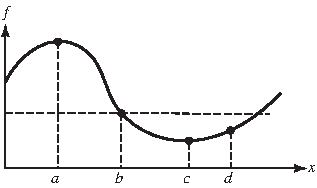
\includegraphics{art/go02m83b}
    \end{problem}

    \begin{solution}
      Since $f(b) < f(a)$, $f(b) - f(a)$ is negative. Similarly, $f(b) - f(c)$ and $f(d) - f(c)$ are positive. So, $f(b) - f(a)$ is the smallest.

      Graphically, $f(b) - f(c)$ represents the vertical distance between $f(b)$ and $f(c)$, and $f(d) - f(c)$ represents the vertical distance between $f(c)$ and $f(d)$. We can see that the first distance is greater, so we get the ordering $\boxed{\text{A} < \text{C} < \text{B}}$.
    \end{solution} 

  \item

    \begin{grading}
      4 points: 1 for knowing $\text{A} = \text{B}$, 1 for knowing
      $\text{D}$ is greatest, 1 for knowing $\text{A} < \text{C}$, 1
      for knowing $\text{C} < \text{E}$. If no explanation, give half credit. 
    \end{grading}

    \begin{problem}[\vfill\newpage]
      \begin{enumeratecols}[label=\Alph*., ref=\Alph*]{5}
      \item $\dfrac{f(b)-f(a)}{b-a}$
      \item $\dfrac{f(a)-f(b)}{a-b}$
      \item $\dfrac{f(c)-f(b)}{c-b}$
      \item $\dfrac{f(d)-f(c)}{d-c}$
      \item $\dfrac{f(d)-f(b)}{d-b}$
      \end{enumeratecols}

      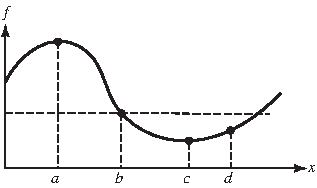
\includegraphics{art/go02m83b}
    \end{problem}

    \begin{solution}
      We can visualize $\dfrac{f(b)-f(a)}{b-a}$ as the slope of the secant line between $(a, f(a))$ and $(b, f(b))$. Similarly, we can visualize all of the other expressions as slopes of secant lines. If we draw these secant lines on the graph of $f$, we see that only D is positive.

      Among the rest, A and B are equal to each other and are the most steep, and E is the least steep; C is in between. Since these are all negative values, A and B are the most negative. So, we get the ordering $\boxed{\text{A} = \text{B} < \text{C} < \text{E} < \text{D}}$.
    \end{solution}

  \end{enumerate}

\item \label{gottlieb-2.3.12-modified} %(2.3.12 revised)

  A bicyclist does a one-mile climb at a constant speed of 12 miles per hour, followed by a one-mile descent at a constant speed of 30 miles per hour.

  \begin{enumerate}
  \item \label{gottlieb-2.3.12b}

    \begin{grading}
      2 points: 1 for correctly calculating the total time, and 1 for using that to get the right average speed. It's okay if they use different units, like $\frac{2}{7}$ miles per minute. If they don't include units, deduct 0.5 points. 
    \end{grading}

    \begin{problem}[\vfill]
      What is her average speed for the two miles? Be sure to explain how you get your answer, and include units with your answer. 
    \end{problem}

    \begin{solution}
      It takes the cyclist $\dfrac{1 \text{ mile}}{12 \text{ miles per hour}} = \dfrac{1}{12}$ hours to reach the top and another $\dfrac{1 \text{ mile}}{30 \text{ miles per hour}} = \dfrac{1}{30}$ hours to go down the hill. So, the total time the cyclist rides is $\dfrac{1}{12} + \dfrac{1}{30} = \dfrac{7}{60}$ hours.

      The average speed is $\dfrac{\text{distance}}{\text{time}} = \dfrac{2 \text{ miles}}{\frac{7}{60} \text{ hours}} = \boxed{\frac{120}{7} \text{ miles per hour}}$. (This is about 17.14 mph.)
    \end{solution} 

  \item

    \begin{grading}
      3 points: 0.5 for choosing the correct graph, 1 for a good explanation of why this graph is correct, 0.5 for correctly labeling the values on the vertical axis correctly, 1 for correctly labeling the values on the horizontal axis. Again, they may use different units. 
    \end{grading}

    \begin{problem}[\stretch{0.5}]
      Which of the following shows the distance the cyclist has traveled as a function of time? Explain your choice, and label the important values on the axes (which are marked for you already).

      \begin{imagetable}{2}{\Alph}
        \begin{tikzpicture}
          \begin{axis}[width=2.5in, height=1.5in, xtick={0.0833, 0.11667}, tick style={red, very thick}, major tick length=0.25cm, xticklabel={$$}, xmax=0.15, ytick={1}, yticklabel={$\qquad$}, ymin=0]
            \addplot+[sharp plot] coordinates { (0, 0) ({1/12}, 1) ({7/60}, 0)};
          \end{axis}
        \end{tikzpicture} &
        \begin{tikzpicture}
          \begin{axis}[width=2.5in, height=1.5in, xtick={0.0333, 0.11667}, 
            tick style={red, very thick}, major tick length=0.25cm, 
            xmax=0.15, ytick={15, 30}, xticklabel={$$}, 
            yticklabel={$\qquad$}, ymin=0]
            \addplot+[sharp plot] coordinates { (0, 0) ({1/30}, 15) ({7/60}, 30)};
          \end{axis}
        \end{tikzpicture} 
        \vspace{16pt} \\
        \begin{tikzpicture}
          \begin{axis}[width=2.5in, height=1.5in, xtick={0.0333, 0.11667}, tick style={red, very thick}, major tick length=0.25cm, xmax=0.15, ytick={12, 30}, xticklabel={$$}, yticklabel={$\qquad$}, ymin=0] %
            \addplot+[sharp plot] coordinates { (0, 12) ({1/30}, 12)}; %
            \addplot+[sharp plot] coordinates { ({1/30}, 30) ({7/60}, 
              30)}; %
            \addplot+[open] coordinates {({1/30}, 12)}; %
            \addplot+[closed] coordinates {({1/30}, 30)}; %
          \end{axis}
        \end{tikzpicture} &
        \begin{tikzpicture}
          \begin{axis}[width=2.5in, height=1.5in, xtick={0.0833, 0.11667}, tick style={red, very thick}, major tick length=0.25cm, xmax=0.15, ytick={1, 2}, xticklabel={$ $}, yticklabel={$\qquad$}, ymin=0] %
            \addplot+[sharp plot] coordinates { (0, 0) ({1/12}, 1) ({7/60}, 2)};
          \end{axis}
        \end{tikzpicture}
      \end{imagetable}
    \end{problem}

    \begin{solution}
      Since this is a graph of distance traveled as a function of time, the 
      function should always be increasing,
      and the slope should represent the speed of the cyclist.
      
      When the cyclist is climbing at a constant speed of 12 miles per hour, the graph has slope 12. After this, the graph has slope 30 since the cyclist is going at a constant speed of 30 miles per hour. So, this must be graph \fbox{D}.

      We found all the important values in \ref{gottlieb-2.3.12b}:
      \begin{center}
        \begin{tikzpicture}
          \begin{axis}[ xtick={.083, 0.11667}, xticklabels={$\dfrac{1}{12}$, $\dfrac{7}{60}$}, ytick={-5, -4, ..., 5}, xlabel={$t$ (hours)}, ylabel={distance (miles)}, xmin=0, xmax=.15, ymin=0, width=3in, height=2in]
            \addplot+[domain=0:1/12] {12*x};
            \addplot+[domain=1/12:.116] {30*x-1.5};
          \end{axis}
        \end{tikzpicture}
      \end{center}
    \end{solution}

  \item \label{gottlieb-2.3.12b-reflect-back}

    \begin{grading}
      1 point. Any reasonable explanation gets full credit. 
    \end{grading}

    \begin{problem}[\nstretch{0.5}]
      \textbf{Reflect Back.} Your friend is working on
      \ref{gottlieb-2.3.12b} and says, ``Since the bicyclist travels
      at 2 speeds, 12 mph and 30 mph, her average speed should just be
      the average of those, which is $\frac{12 + 30}{2} = 21$ mph.''
      However, your friend's answer is incorrect! Explain to your
      friend \emph{why} their reasoning is incorrect.
    \end{problem}

    \begin{solution}
      You can't just average the two speeds because that doesn't take
      into account how long the bicyclist traveled at each speed.
      Average speed is distance traveled divided by elapsed time.
    \end{solution}

  \end{enumerate}

\item  
  \begin{grading}
    Nothing to turn in
  \end{grading}

  Start working on Practice Mini-Exam 1; if you didn't pick up a copy in class, you can find one on the Exams page of Canvas. See the practice exam for more detailed instructions. We'll cover the material for \#5 on Wednesday, so we recommend waiting until after Wednesday's class to do \#5. 

\end{enumerate}
\psreflection{For next class, read pg. 126 - 129 of \S 3.4.}
\end{document}
